\documentclass{acm_proc_article-sp}
\usepackage{graphicx}
\usepackage{hyperref}
\usepackage{amsmath}
\usepackage{float}
\usepackage{caption}

\makeatletter
\def\@copyrightspace{\relax}
\makeatother

\begin{document}
%work on this title
\title{Reflections On Project 1}
\subtitle{Feature Extractions, Bad Smells, and How to Detect Them Early \thanks{This report is Group G's May 1 Deliverable for CSC 510 taught by Dr. T. Menzies in the Spring of 2016 at North Carolina State University.}}

\numberofauthors{4} 
\author{
\alignauthor
Brian Clee\\
       \email{bpclee@ncsu.edu}
\alignauthor
Effat Farhana\\
       \email{efarhan@ncsu.edu}
\and % go to new row
\alignauthor
Arjun Madan\\
       \email{amadan2@ncsu.edu}
\alignauthor
Ran Tan\\
       \email{rtan2@ncsu.edu}
}

\date{7 April 2016}
\maketitle

\begin{abstract}
One of the unique aspects of collaborating on group projects through GitHub is the public access of nearly all collaboration data. These data artifacts can in turn be mined and categorized into sets of small features which can demonstrate and visualize how groups work together. We have done precisely this for six CSC 510 project groups, including our own, defining 10 small features and performing rigorous data analysis on them. Further we have determined 6 bad smells of group collaboration failures and demonstrated how each of these six groups exhibits, or doesn't exhibit, these bad smells. Finally, we have discussed an early bad smell detection system which would take a group's data at chronological points to determine which bad smells are most likely to occur and what to look out for.

\end{abstract}

\section{Introduction}\label{sec:intro}

Throughout this semester groups of CSC 510 students have been collaborating on GitHub to complete their semester projects. While working through GitHub, these groups, and us included, have been leaving a wealth of data that reflects our team dynamics, work schedules, and overall progress. This data presents itself in many forms but mainly falls into the categories of issues, milestones, comments, and commits. These data artifacts are discussed in section~\ref{sec:datacollect} where we discuss our retrieval processes for gathering this data in more detail.

From these mine-able data artifacts we can then explore how the different groups work together. We go on to define a set of 10 small features gathered from this data and discuss them in section~\ref{sec:smallfeatures}. Here we define different metrics of combining our data to observe quantitative features of how each group works together.

After determining how groups work together, we then address the arguably more important topic of discovering how they don't work together. This idea of observable negligence will be generally referred to as "bad smells", and by coming up with 6 metrics to define these bad smells we can declare which groups worked best and worst together throughout the semester. We discuss our bad smell detection methods in section~\ref{sec:smelldetect}.

Furthermore, by defining bad smells and how to detect them, we can also come up with a system to detect bad smells early in a group's work cycle. We discuss this early bad smell detector system in section~\ref{sec:earlydetect}. Due to time constraints we did not actually develop such a system, but did perform background research on what it would take to create one, and the features it would need to include.

\section{Data Collection}\label{sec:datacollect}
The data we collected for sections~\ref{sec:smallfeatures},~\ref{sec:smelldetect}, and~\ref{sec:earlydetect} included all the public issues (including pull requests), comments, commits, and milestones for six CSC 510 project groups, referred to as Groups 1 through 6 for anonymization purposes.

All the data was collected using a modified version of the ``gitable'' script written by a group from the Spring 2015 version of the CSC 510 course~\cite{Axitron}. The script made GET requests to the official GitHub API~\cite{githubapi} which returned information about a particular group's repository's issues, comments, commits and milestones. All the relevant information was then stored in an SQLite database which was then later extracted for analysis. 

One of the major changes we were forced to make to this script was due to an interesting error that seemed to plague many of the repositories for this years groups. Essentially, whenever a user had login information that was not present, or if they had an unverified email address, they would show up as multiple users instead of one. Because of this the script was modified to allow us to collect data when user login information was not present, combining the multiple "ghost" users into a single entity.

The fields of the data that we stored were organized into four major categories: issues, milestones, comments, and commits. For issues we stored the issue ID, issue name, creation time, action performed, and user associated with the action. For milestones we stored the milestone ID, description, creation time, due time, closed time, and the user who originally created it. For comments we stored the user, the issue the comment was on, timestamp, and text of the comment. And finally, for commits we stored the user, timestamp, message, and also the number of changes the commit had.

The data was then extracted from the SQLite database and transformed such that we could analyze it. The transformed data was stored in CSV files, which were used to generate the graphs we see in section~\ref{sec:smallfeatures} using R~\cite{rcite}. This transformation was done through shell scripts which ran various SQLite commands to group rows by user, and selected only the fields that pertained to a certain feature, thus creating a unique CSV for each feature that we cared about.

The data was also anonymized by looking at the login information of the owner of the data, and replacing it with a generic unique name (such as user1, user2, etc.). As discussed previously, one problem we faced while anonymizing the data was that some of the commits did not have any login information associated with it. As we discussed this was due to the user not having linked their email address correctly with the commit. This prevented us from getting correct data from many of the groups. For example, our group also faced this issue, but since we knew the cases where the login information was missing, it was easy to include a fix in the script, which involved adding the login information externally when it was missing.

As discussed earlier, the data was also further anonymized throughout our figures such that rather than referring to a group's actual name, they are referred to by a random number. All of our figures in this report follow this convention so as to not call out other classmates specifically by name.

\section{Small Features Detection}\label{sec:smallfeatures}

Complex patterns are based on small features. To have a better understanding of the working pattern of each group, we come up with a couple of small features to describe the behavior of each group on GitHub. First, we summarize and compare the basic statistics of each group on issues, comments, milestones and commits. Then, we discuss these features from four aspects, namely, progress, communication, collaboration and effectiveness.


\subsection{Data Summary}

In this section we look at the total number of comments, commits, issues, and milestones created by the six groups whose data we've collected.

We hypothesize that groups that have more comments, commits, issues and milestones have members that communicate better, and work together more efficiently. These are the groups where the probability of all members having an equal contribution to the project is higher.

\subsubsection{Total Number of Comments}
Figure \ref{fig:grComment} shows us that Group 4 had the maximum number of comments with 253, while Group 2 were slightly further behind with 138, and Groups 1, 5, and 6 had the fewest comments. Group 1 had the fewest with there being only 25 comments on their issues. 

\begin{figure}[h]
\centering
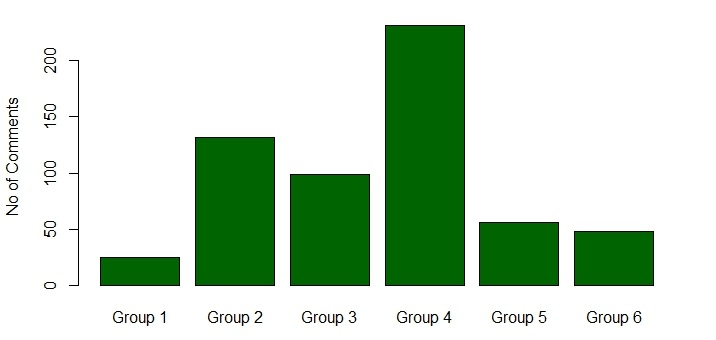
\includegraphics[width=8cm]{img/grComment}
\caption{Total Comments Per Group}
\label{fig:grComment}
\end{figure}

\subsubsection{Total Number of Commits}
Figure \ref{fig:grCommit} shows us that Group 2 had the maximum commits with 225. Group 4 had the second highest number of commits with 177, while Groups 1, 3, 6 had slightly fewer. Group 5 had the lowest number of commits with just 77. 

\begin{figure}[h]
\centering
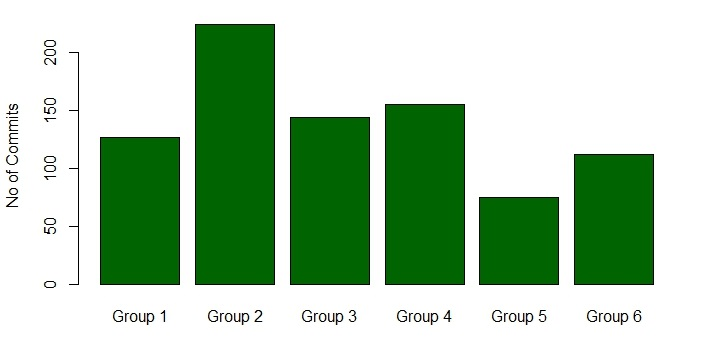
\includegraphics[width=8cm]{img/grCommit}
\caption{Total Commits Per Group}
\label{fig:grCommit}
\end{figure}

\subsubsection{Total Number of Issues}
Figure \ref{fig:grIssue} shows us that Group 3 and Group 4 had the maximum number of issues with just over 80. Group 2 were just behind had around 60 commits. Group 1 had the least issues with around 35. This, along with the the fact that they had the lowest number of comments shows us that there wasn't a lot of communication or collaboration between the members here.

\begin{figure}[h]
\centering
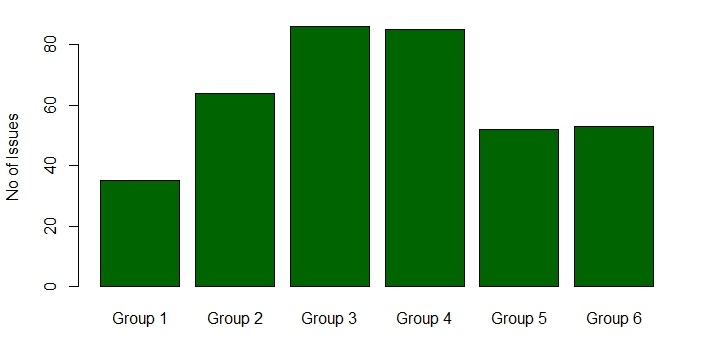
\includegraphics[width=8cm]{img/grIssue}
\caption{Total Issues Per Group}
\label{fig:grIssue}
\end{figure}

\subsubsection{Total Number of Milestones}
Figure \ref{fig:grMilestones} shows us that Group 6 created the most milestones with more than 16. Group 1 were second with 14. Group 3 had the least milestones with just 7. This shows us that Group 3 perhaps did not divide their work into blocks that had to be worked on over time. An interesting thing of note here is that Group 1 had the most milestones with the least issues, which indicates their members tended to largely work on their own, and there wasn't a lot of collaboration between them.

\begin{figure}[h]
\centering
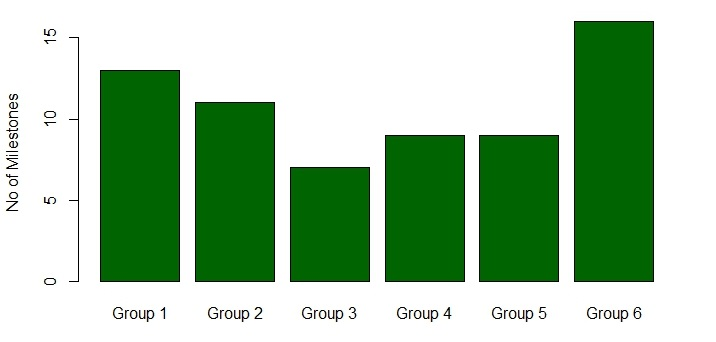
\includegraphics[width=8cm]{img/milestone}
\caption{Total Milestones Per Group}
\label{fig:grMilestones}
\end{figure}

\subsection{Progress}

Now that we have summarized the data generally, we will begin going over our ten small features we have identified. To make things easier to understand and follow, we have further broken these ten features down into context groups.

The first group of features we will discuss relates to a group's progress towards their goals. Here we are concerned with whether or not they are making significant progress throughout the semester.

\subsubsection{Issues Closed Per Week}
Figure \ref{fig:closedPerWeek} shows us how many issues were closed each week. The X-axis shows us the week number, where week 1 is the first week an issue was closed, and the last week is when the last issue was closed. Ideally, we'd expect issues closed every week since people should be continuously working on the project, with peaks closer to the deadlines when most work is completed. From the line graphs we see that this is the case with Group 2 and Group 4. Group 5 was also pretty regular with their work except for a three week period towards the end where they did not close any issues. Group 1, 3 and 6 had issues closed only over a 6 to 7 week period and this shows us that they didn't start work with the rest of the groups or they didn't use issues properly to log their work.

\begin{figure}[h]
\centering
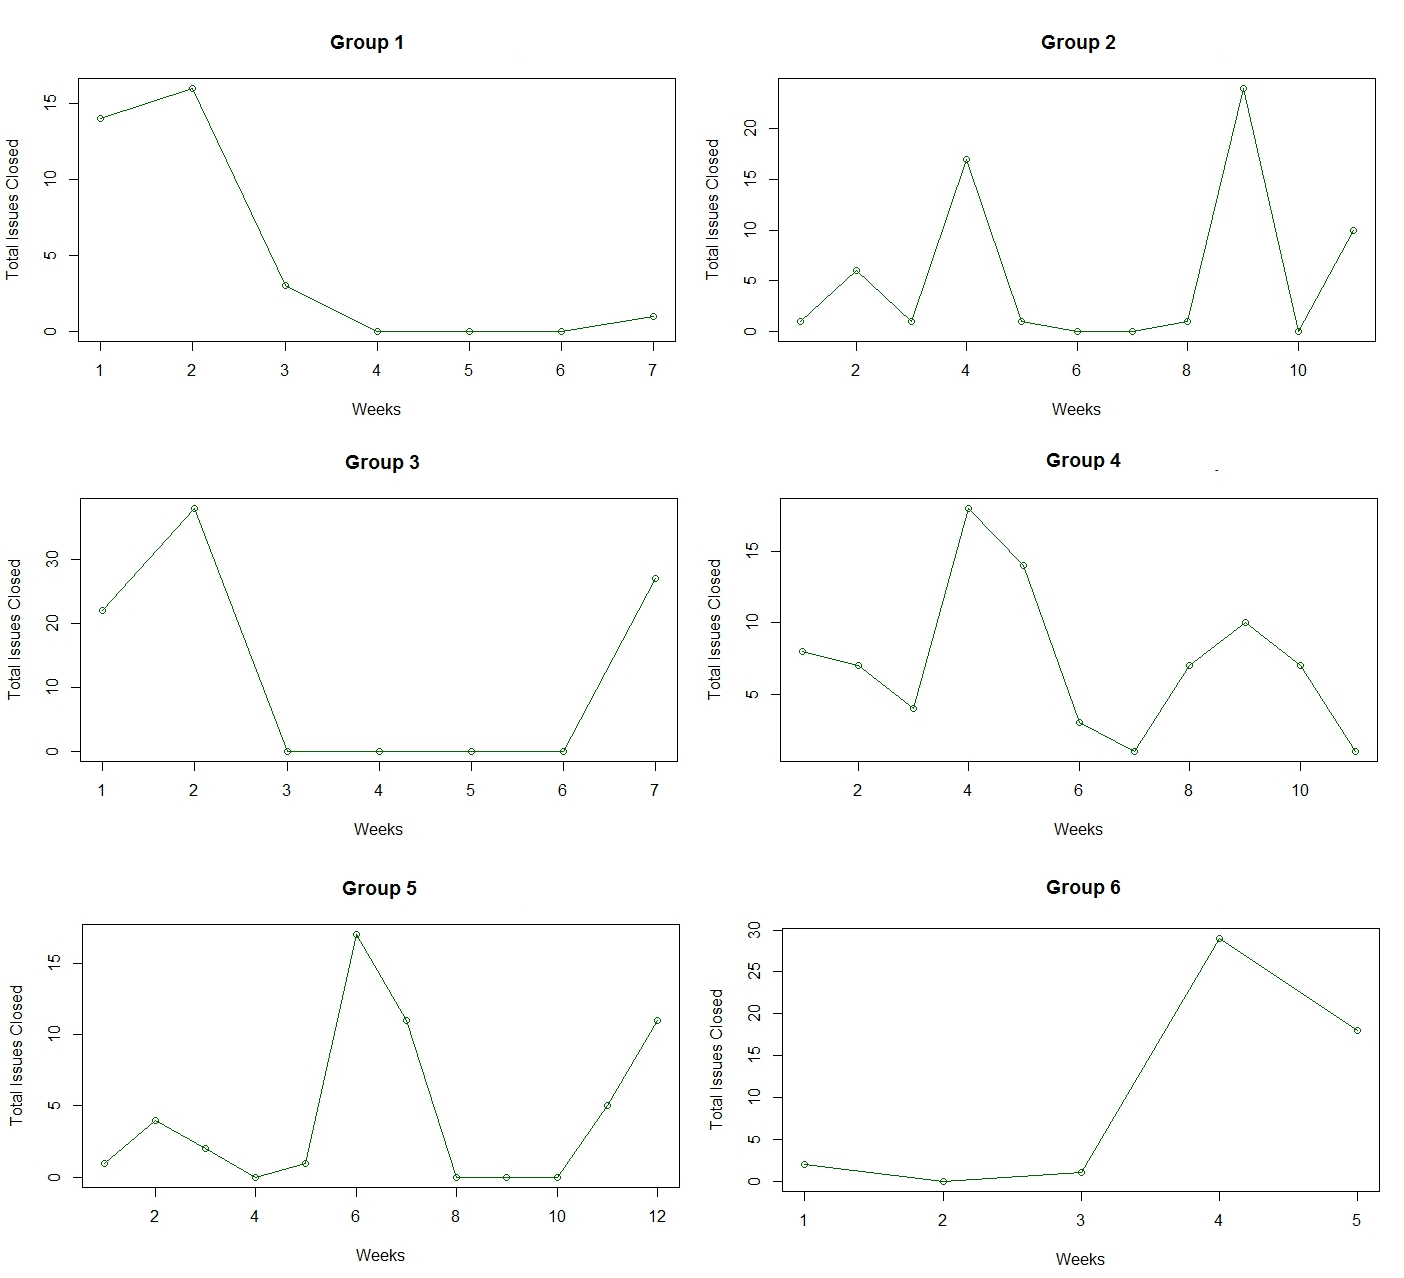
\includegraphics[width=8cm]{img/closedPerWeek}
\caption{Issues Closed Per Week}
\label{fig:closedPerWeek}
\end{figure}

\subsubsection{Commits Per Week}
Figure \ref{fig:commitsPerWeek} shows us the number of commits made by the members of a group over the course of the project. As in the section above, the X-axis shows us the week number, Week 1 is the first week there was a commit. From the line graphs we can see that all groups had a peak around week 7-8 which coincides with the Mar1 deliverable, showing us that most of the work was done closer to the deadline. Group 1 exhibit the most ideal case where the number of commits rises gradually as the deadline approaches, and then peaks the week of the deadline. Group 1, 3, 5, and 6 however experienced a period of 2-4 weeks immediately after the deadline where no new commits where made, and this deviates from what we'd expect in a project that is still continuing.

\begin{figure}[h]
\centering
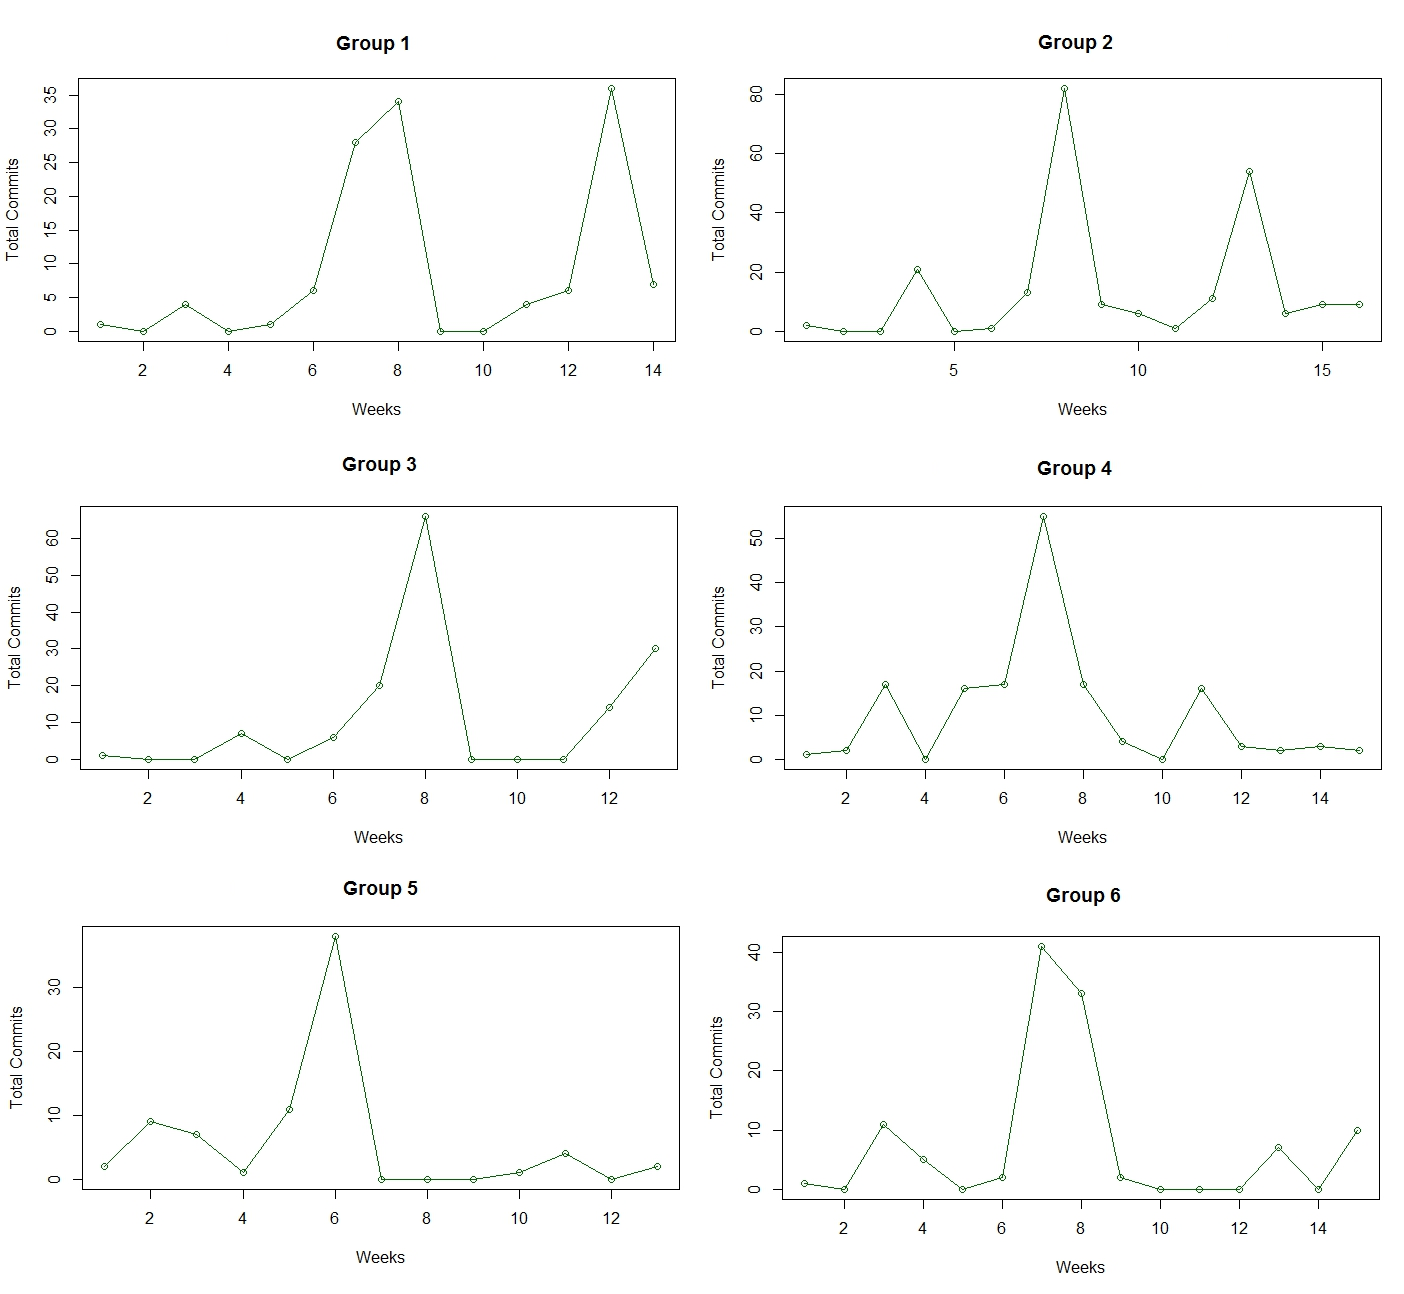
\includegraphics[width=8cm]{img/commitsPerWeek}
\caption{Commits Per Week}
\label{fig:commitsPerWeek}
\end{figure}

\subsection{Communication}

This section talks about the data collected, and graphs constructed for small features related to communication. Ideally a group communicates effectively with each other, where all members are contributing to conversations more or less equally.

\subsubsection{Total Comments Per User}

Figure \ref{fig:comments} shows us the proportion of comments each user of a group made. We would expect each user to contribute approximately the same amount in an ideal situation. The pie charts show us that Group 2 and Group 3 had users commenting almost equally, and these groups are closest to the ideal scenario. Group 4 had user 1 and user 2 commenting almost 75\% of the time. Group 1 and Group 2 had their user 2s contributing to approximately half the number of comments made in their issues. Group 5 actually had user 1 make almost 75\% of the comments, which is definitely not ideal.

\begin{figure}[h]
\centering
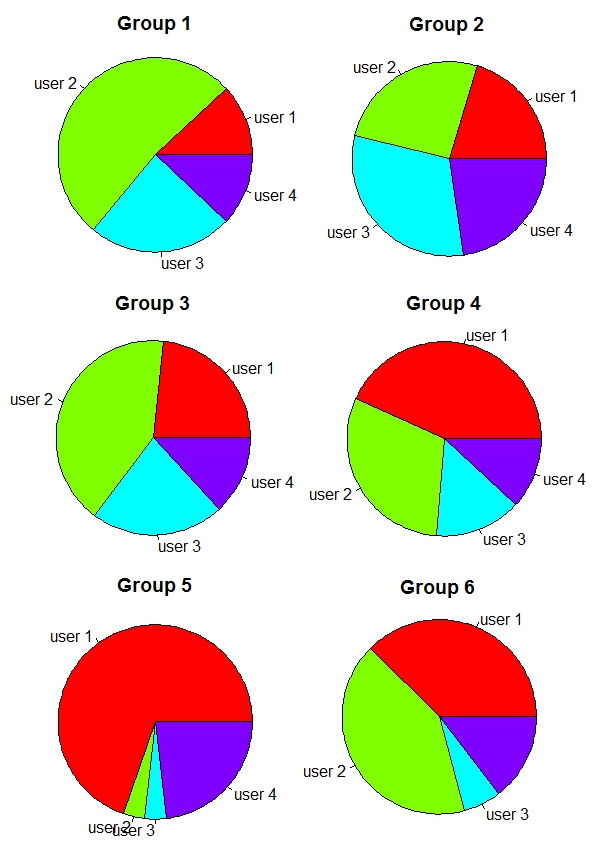
\includegraphics[width=8cm]{img/comment_user}
\caption{Total Comments Per User}
\label{fig:comments}
\end{figure}

\subsubsection{Number of Comments Per Issue}

Figure \ref{fig:numcomments} is a boxplot that shows the number of comments made per issue for the six groups. We hypothesize that groups having a greater number of comments per issue, have more collaboration and better communication among members. From the boxplot we see that Group 2 and Group 4 have the most comments per issue with the median number of comments at 4. This means that for any issue, there was an average of 4 comments made on it. Group 6 on the other hand had a median of 1 comment per issue, and this can be verified by observing that the number of comments is just slightly higher than the number of issues from Figure \ref{fig:grComment} and Figure \ref{fig:grIssue}.

\begin{figure}[h]
\centering
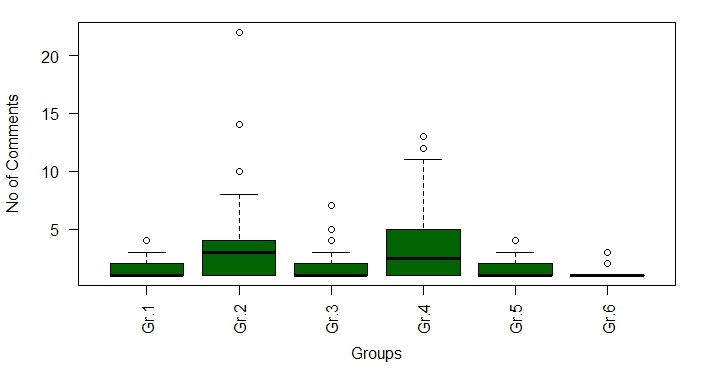
\includegraphics[width=8cm]{img/numcomments}
\caption{Comments on Issues Per Group}
\label{fig:numcomments}
\end{figure}

\subsubsection{Participants Per Issue}

Figure \ref{fig:issueComment} shows us the average of the number of participants on an issue. In an ideal case we'd expect the median to be on 3 or 4 users, since members should ideally be communicating about the issues they face. From the boxplot we see that Group 2 is the closest to this ideal case. Groups 1, 5 and 6 actually have, in most cases, only one user commenting on an issue which indicates there was no proper collaboration or communication when it came to dealing with issues. Group 3 also had a median of 1, but had quite a few issues where there were at least two users commenting. Group 4 was similar, but slightly better with a median of two.

\begin{figure}[h]
\centering
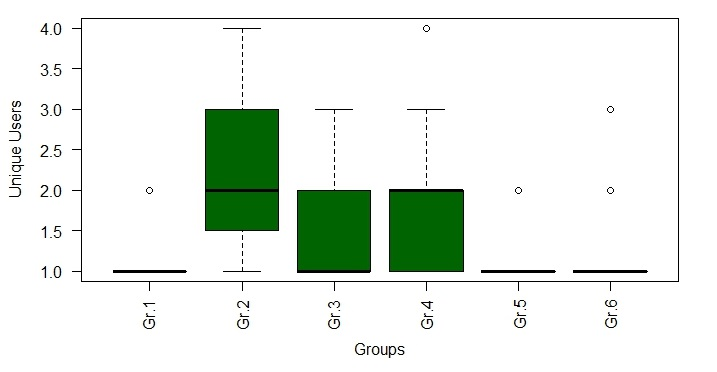
\includegraphics[width=8cm]{img/issueComment}
\caption{Participants Per Issue}
\label{fig:issueComment}
\end{figure}

\subsection{Collaboration}

This section talks about the data collected and graphs constructed for small features related to collaboration. Ideally a group not only communicates well but also collaborates well. That is, they share the work load evenly between themselves.

\subsubsection{Per Issue Assignees}
Figure \ref{fig:assign} shows us the proportion of issues assigned to each user in the group. For any group, we expect the ideal case to be that where every user contributes equally, i.e., has almost the same number of issues assigned to them. From the different pie charts we see that this is largely the case for most groups. Group 4 and Group 6 are cases where this is not true. Group 4 has user 1 with a slightly higher number of issues assigned, while user 3 seems has fewer issues assigned. Group 6 has user 2 with roughly two-third of the issues assigned to them. user 2 doesn't have any issues assigned, while user 3 has less than 10\% of the issues assigned to them. This shows us that user 2 and user 3 did not contribute as much to the project, while user 2 did most of the work. However, we feel this is not an accurate representation of the work break-up as on further analyzing the data, we observed that the number of assignments made were fewer than the number of issues, indicating that assignments were not properly used by the groups.

\begin{figure}[h]
\centering
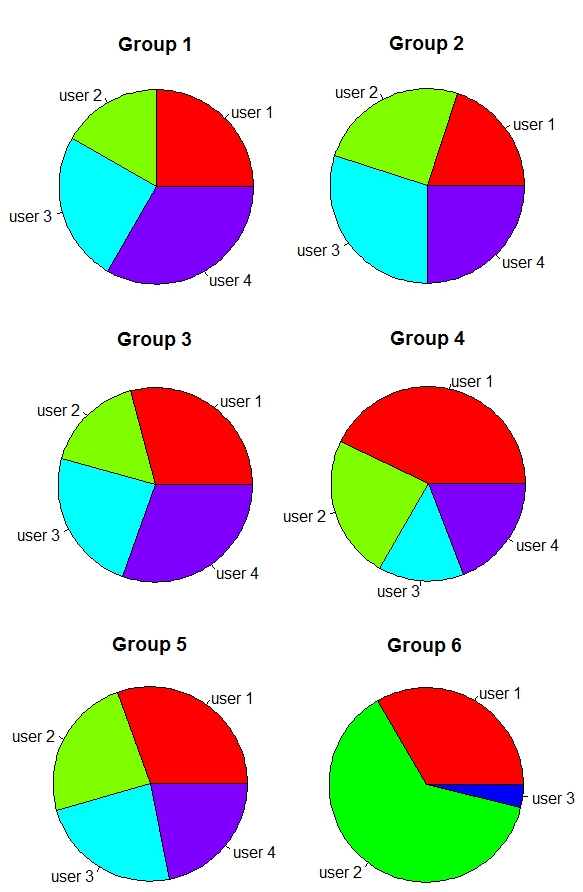
\includegraphics[width=8cm]{img/assignments}
\caption{Issue Assignments}
\label{fig:assign}
\end{figure}

\subsubsection{Number of Changes Per User}
Figure \ref{fig:changes_made} show us the proportion of changes each user in the group made. The total number of changes for this purpose is defined as the difference between the number of additions and number of deletions a user made over the course of the project. We estimated the number of changes to be approximately equal for each member, but found out that wasn't the case in any group. This is because of the way GitHub treats changes with text documents. It treats every line as an addition, and these documents are usually written outside GitHub and then committed by one user, thereby crediting that user with all the additions. As a result we revised our expectations, and just looked for cases where a user was not present, or had a very small final contribution. Group 1 had user 2 and user 4 with an unusually small final contribution to the project, while Group 4 had user 3 and user 4 with an unusually small final contribution. Group 2 had user 1 with an unusually small final contribution. 

\begin{figure}[h]
\centering
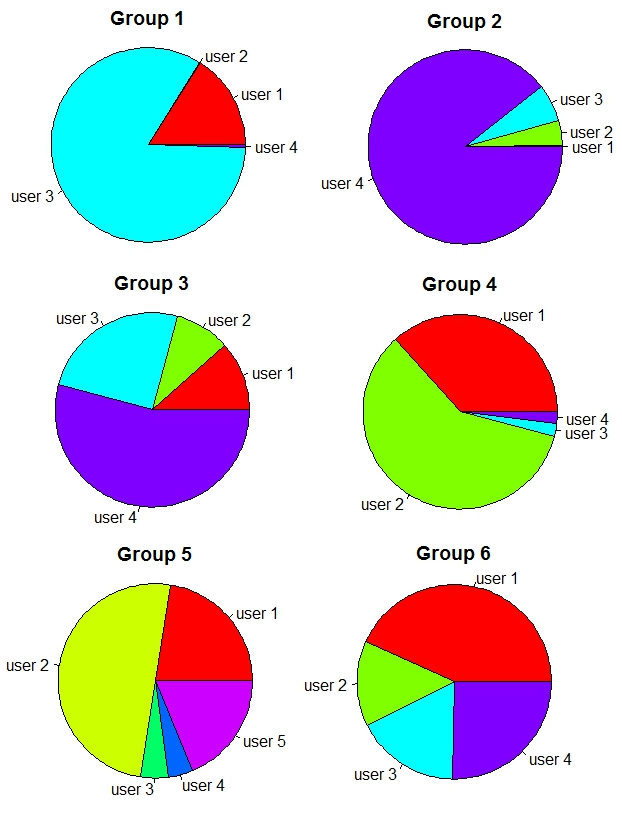
\includegraphics[width=8cm]{img/change_made}
\caption{Total Changes Made Proportionally}
\label{fig:changes_made}
\end{figure}

\subsubsection{Number of Events Per User}\label{sec:events_user}
Figure \ref{fig:issue_create} shows us the number of events each user was a part of. GitHub defines an ``event'' as something that takes place on an issue. It includes labelling, referencing, mentioning, closing, merging, subscribing or unsubscribing to, and milestoning the issue. GitHub also adds an automatic login ``history'' to events when an issue is subscribed to or referenced. This is what is ``user 5'' in our pie charts, and can be ignored for this analysis. 

Again, we would expect all the users to have approximately an even share of events they've contributed to. From the pie charts in Figure\ref{fig:issue_create}, we see that this is the case for Group 2. Group 4 seemed to have user 1 and user 2 take part in about two-thirds of the events, while Group 6 had user 2 take part in more than three-fourths of the events alone. Group 1 also had user 3, and Group 5 had user 2 take part in approximately half the events, indicating that these groups had one member that did most of the work pertaining to organizing issues.

\begin{figure}[h]
\centering
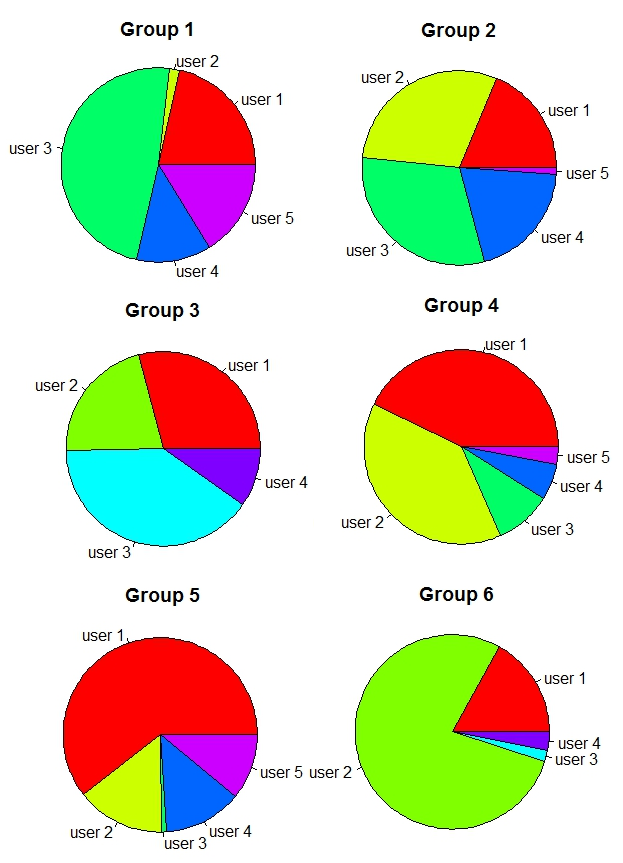
\includegraphics[width=8cm]{img/issue_create}
\caption{Number of Events Per User}
\label{fig:issue_create}
\end{figure}

\subsection{Effectiveness}

\subsubsection{Number of Changes Per Commit}
Figure \ref{fig:commit_changes} shows us the number of changes made per commit. Change here is defined as the difference in the number of additions and deletions per commit. We would expect most of the commits to not be too large, as they are supposed to be used to add small components of the project. We would also expect more commits to be additions since this indicates that the project is progressing. Groups 1, 4, 5 and 6 show this sort of behaviour. Groups 5, and 6 are probably the best of the groups as most of their commits are small, with only a few larger ones. Moreover, there are no major deletions which show that their commits were effective.

\begin{figure}[h]
\centering
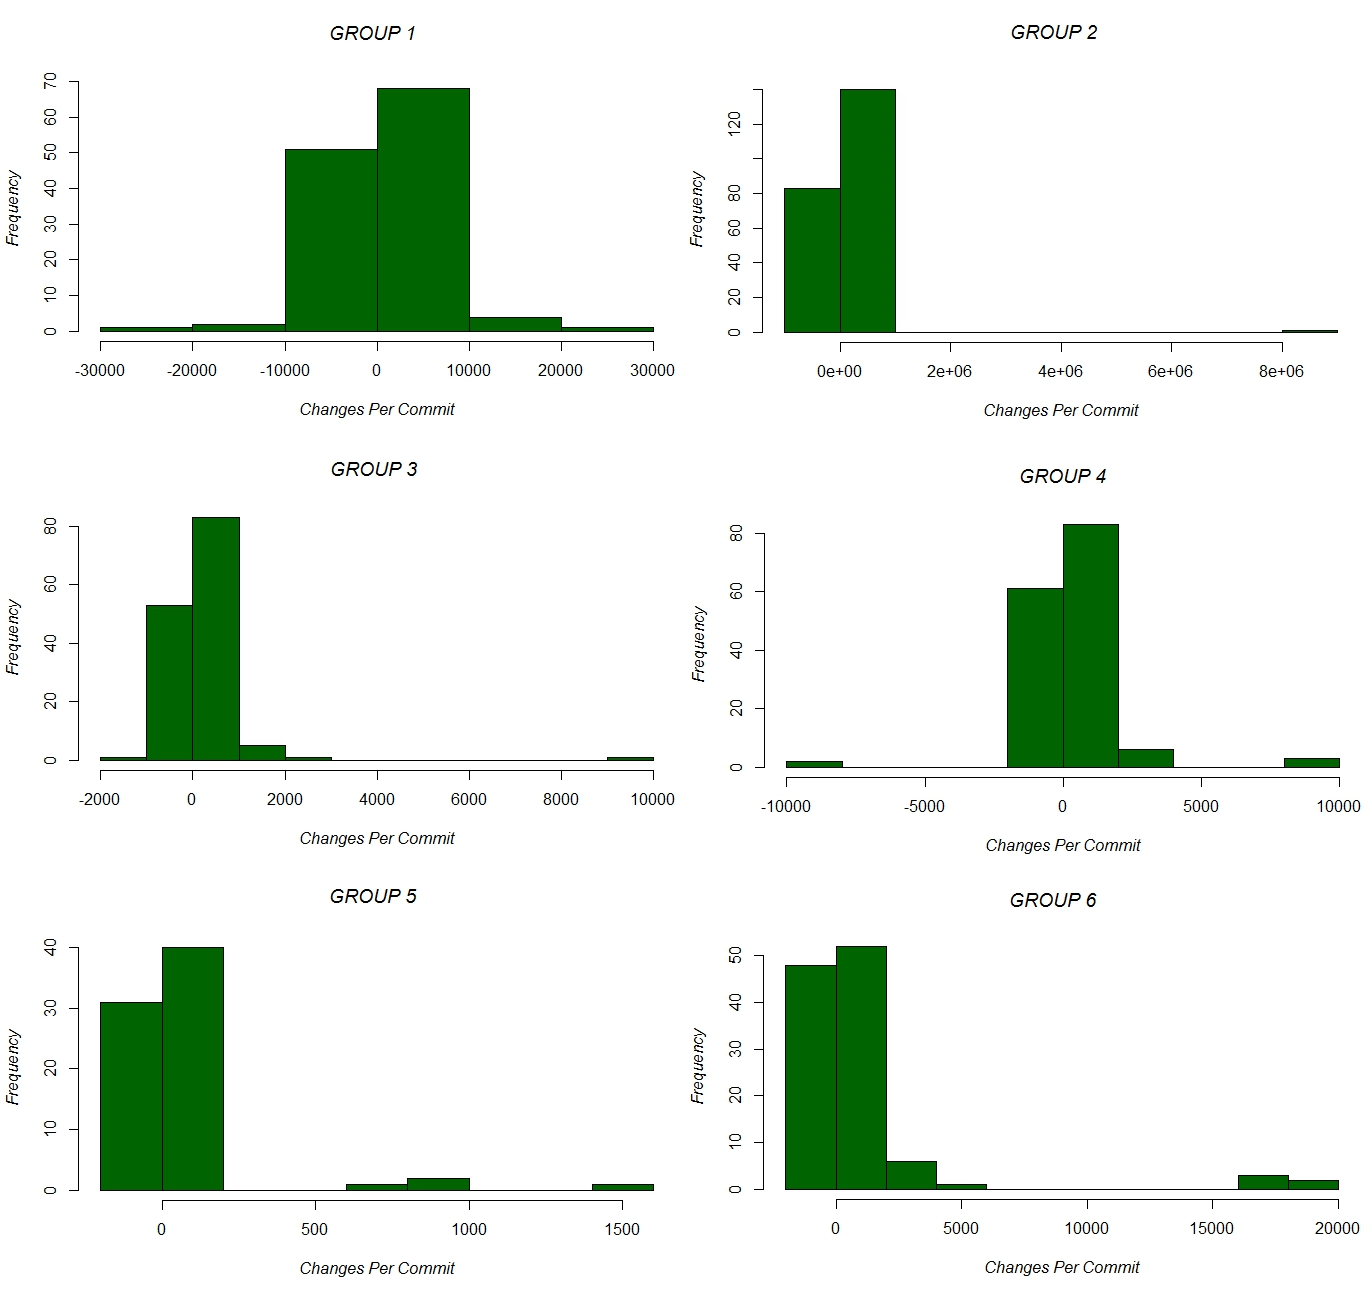
\includegraphics[width=8cm]{img/changed_per_commit}
\caption{Total Changes Per Commit}
\label{fig:commit_changes}
\end{figure}

\subsubsection{Bug Issues}

Figure \ref{fig:bugfix} shows us the proportion of issues that had labels that indicated there was a bug that had been found. Having no bugs found, or having too many issues labelled with terms pertaining to bugs raises questions with a project's progress and effectiveness. If there were no issues that had a label indicating there is a bug, one possibility is that the group didn't test enough. Another possibility is that the group didn't use issues to communicate on the presence of bugs in the code. 

On the other hand, having too many bugs, also indicates that something isn't quite right with the project. Both these cases lead to a drop in effectiveness of the development of the project. The pie chart shows us that Group 1 reported no bugs through issues, while Group 5 and Group 6 had an unusually high proportion of issues that were related to bugs. Group 1 also had the least number of issues, indicating they did not really use them correctly. This is one possible reason for the lack of any issues being related to bugs. Groups 2, 3 and 4 had approximately 5\% of their issues related to bugs, and this seems to be a reasonable number to indicate their projects were progressing smoothly.

\begin{figure}[h]
\centering
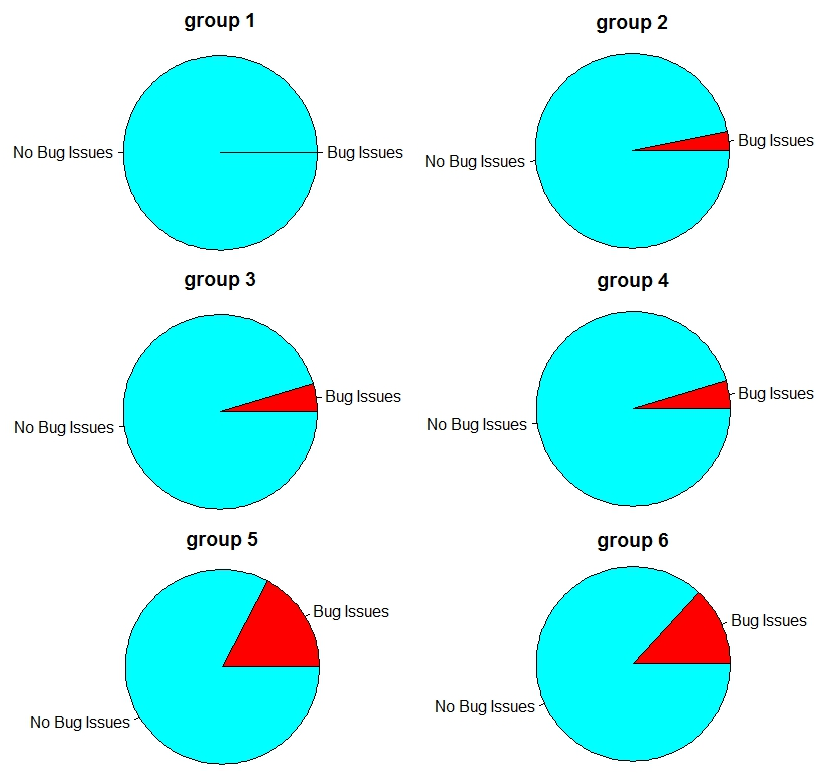
\includegraphics[width=8cm]{img/bugratio}
\caption{Number of Bug Issues}
\label{fig:bugfix}
\end{figure}

\section{Bad Smell Detection}\label{sec:smelldetect}

According to~\cite{tufano2015and}, bad smells in programming are "symptoms of poor design and implementation choices".  Martin Fowler~\cite{Martin} further points out that "a code smell is a surface indication that usually corresponds to a deeper problem in the system". The definition indicates two aspects of "a bad smell": it should be quick to spot and it should most of time lead to interesting problems upon further inspection. 

Unlike the convention where bad smells are detected by analyzing source code and used for code refactoring, here we adopted a different approach by analyzing the GitHub data generated along with the development process and focused on its implication of problems with design and development. With the statistics and data analysis on small features we already have in section~\ref{sec:smallfeatures}, in this section we will discuss bad smells as combinations of our feature extractors.

\subsection{Progress}

In continuing with the same organization of our small features, we will discuss our bad smells within the context of their parent category.

When looking at figures~\ref{fig:closedPerWeek} and~\ref{fig:commitsPerWeek} and considering a group's progress we can notice two different bad smells. The first is doing a lot or most of the work up front, and then forgetting about the project until deadlines. Alternatively, the second bad smell is waiting until right before a deadline to do all of the work. 

It's important to realize that the second deliverable was the most intensive as far as work needed, or code that had to be submitted. For this reason in every single group shown in figure~\ref{fig:commitsPerWeek} there is a peak around the seventh week. 

However, when observing groups 1 and 3, we can see from both of these figures that after submitting their first deliverable their progress halted to a stop and no work was completed or communicated until right before the next submission three weeks later. This is a clear example of the first bad smell where these groups failed to start early on their projects, and instead waited until deadline pressure to start working.

On the other hand, if we observe group 6 we can see an example of the second bad smell, where they had poor communication as seen in figure~\ref{fig:closedPerWeek} which led them to submit most of their commits right before a deadline as seen in figure~\ref{fig:commitsPerWeek}.

\subsection{Communication}

For communication we defined a single major bad smell to be one sided communication. This bad smell corresponds to a singular user in the group communicating solely to themselves. We can see this when a group's issues are mainly composed of just one participant, or when the total comments per user are particularly lopsided.

The major groups that stand out for this bad smell are groups 1, 5, and 6. When we look at figure~\ref{fig:grComment} we can immediately see that of all the groups these three group had by far the least communication through comments. Furthermore, when we cross reference this knowledge with figure~\ref{fig:comments} we can confirm that in the case of groups 1 and 5, a singular user is doing the majority of commenting. This is a clear example of our bad smell of one sided communication.

Alternatively, another form of this bad smell exists and is demonstrated by group 6, wherein two different users are engaging in one sided communication. We can confirm that this is still one sided communication by looking at figure~\ref{fig:issueComment} which shows that for groups 1, 5, and 6, they all on average have a single participant commenting on their issues with outliers of 2 and 3. This shows that one sided communication doesn't just occur when only one person is doing the majority of the communication, but can also occur when two people are the majority communicators, however, they are only communicating with themselves.

\subsection{Collaboration}

In terms of collaboration the major bad smell we identified was having a one person team. This obviously occurs when one person on the team does the majority of the work both through the changes they make in their commits and events they contribute to the project.

To demonstrate this, figure~\ref{fig:changes_made} displays the changes made proportionally by user to the code base through commits, and figure~\ref{fig:issue_create} displays the events proportionally by user (see section~\ref{sec:events_user} for more information on what classifies an event). When looking at these two figures we can see a trend with groups 1, 5, and 6 identifying them as examples of one person teams.

Take for example figure~\ref{fig:changes_made}, which shows that an overwhelming majority of the changes made for group 1 were by a single person. As well, groups 5 and 6 also demonstrate a single person doing most of the changes.  We must next cross reference figure~\ref{fig:issue_create} to affirm these findings and we can see that for groups 1, 5, and 6 the majority of events are also done by the same user. Its necessary to make this cross reference, otherwise if we just look at changes made it would appear more groups classify as one person groups, when in reality the entire group is working together, rather a single user happens to have proportionally more commits.

When inspecting these two figures with this bad smell, it is also important to identify a sub bad smell, the two person group. An example of for this smell is group 4, which as shown in figures~\ref{fig:changes_made} and~\ref{fig:issue_create} exhibit two users doing the majority of changes and events. 

Along with this bad smell of one and two person groups there is also another bad smell that can be identified within these figures that we call, communication without collaboration. An example of this bad smell can be seen with group 2. In figure~\ref{fig:issue_create} we can see that group 2 has excellent collaboration through events, and if we back reference to figure~\ref{fig:comments} they also have excellent communication. However, when observing figure~\ref{fig:changes_made} it is apparent that a single user did most of the changes through commits. Thus group 2 is an example of communicating without collaborating.

\subsection{Effectiveness}

On effectiveness we define a group's commits to be effective when they commit frequent small changes to the code base that don't introduce bugs. To this end, we have defined two bad smells on effectiveness. 

The first bad smell is the waterfall commit. This occurs when a group spends way too much time working on the code base in a single commit, making gigantic and disproportional additions with no deletions to match. Furthermore we coined this term as waterfall because even though they contributed everything in one large batch, they also spent a lot of time bug testing their bulk addition. 

A group that demonstrates this bad waterfall commit smell is group 2. If we look at figure~\ref{fig:commit_changes} we can see that group 2 had the majority of their commits in a reasonable neighborhood of small additions and deletions; however, they also had one absurdly large addition that was not counterbalanced by a deletion. Further, if we cross reference this with figure~\ref{fig:bugfix} we can see that this gigantic addition did not introduce as many bugs as it should have. Therefore, group 2 is a clear example of a bad waterfall commiter.

On the other hand, our second bad smell related to effectiveness is untested large commits. This occurs when a group semi-frequently adds larger commits than their normal sizes and does not efficiently bug test these commits. Examples of this bad smell can be seen by looking at groups 5 and 6, we can see in figure~\ref{fig:commit_changes} that both of these groups have semi-frequent larger than normal commits without appropriate deletions to counter balance them. As well, when we then look at figure~\ref{fig:bugfix} we see that both of these groups had the largest bug issues introduced from their changes. Thus, both groups 5 and 6 fall victim to the untested large commits bad smell.

\section{Early Bad Smell Detector}\label{sec:earlydetect}

Bad smells are easy to spot and more often than not lead to problems beneath the surface. However, they rely on features that can only be observed after the process of design and development. This limitation of bad smells prevents us from detecting underlying problems with design and development before the delivery of software and predicting negative consequences to avoid possible loss to the project. To address this challenge to the effectiveness of a bad smell detector, we sorted the data chronologically and devised a modified mechanism based on reasonable assumptions. This provides as an immediate feedback on the progress and allows us to predict underlying problems with the software along with the process of design and development.

The first question comes to us is how much data is enough for evaluating whether the whole project is going in the right direction. To answer this question, we have to look into figure~\ref{fig:closedPerWeek}and figure~\ref{fig:commitsPerWeek} for the progress of the project. The statistics indicate that the first four weeks is informative enough to predict the rest of the project. So we choose the first four week as our sample data for early bad smell detection.

With further inspection into figure~\ref{fig:closedPerWeek} and figure~\ref{fig:commitsPerWeek}, we can find some interesting patterns. If one group closed a lot of issues (say above 15) and showed a decline in the first four weeks, they probably wouldn't make much progress later. On the other hand, if a group didn't close enough issues (say below 5) in the first few weeks, it's very likely that they were behind their schedule and would have lots of commits right before the submission deadline. 

This analysis coordinates with our conclusion in section~\ref{sec:smelldetect} that group 1 and 3 doing most of the work upfront and put is aside until the next deadline; also that group 6 always wait until the last minute. To justify this analysis, there are two underlying assumption. Namely that it takes similar amount of time and effort among groups to work on the project, and that the working pattern on the project remain the same. So if one group did most of the job at the beginning, they wouldn't make much progress later, vice versa. The early bad smells are shown in figure~\ref{fig:closedDetect} via a red line to signify when the groups got off track.

\begin{figure}[h]
\centering
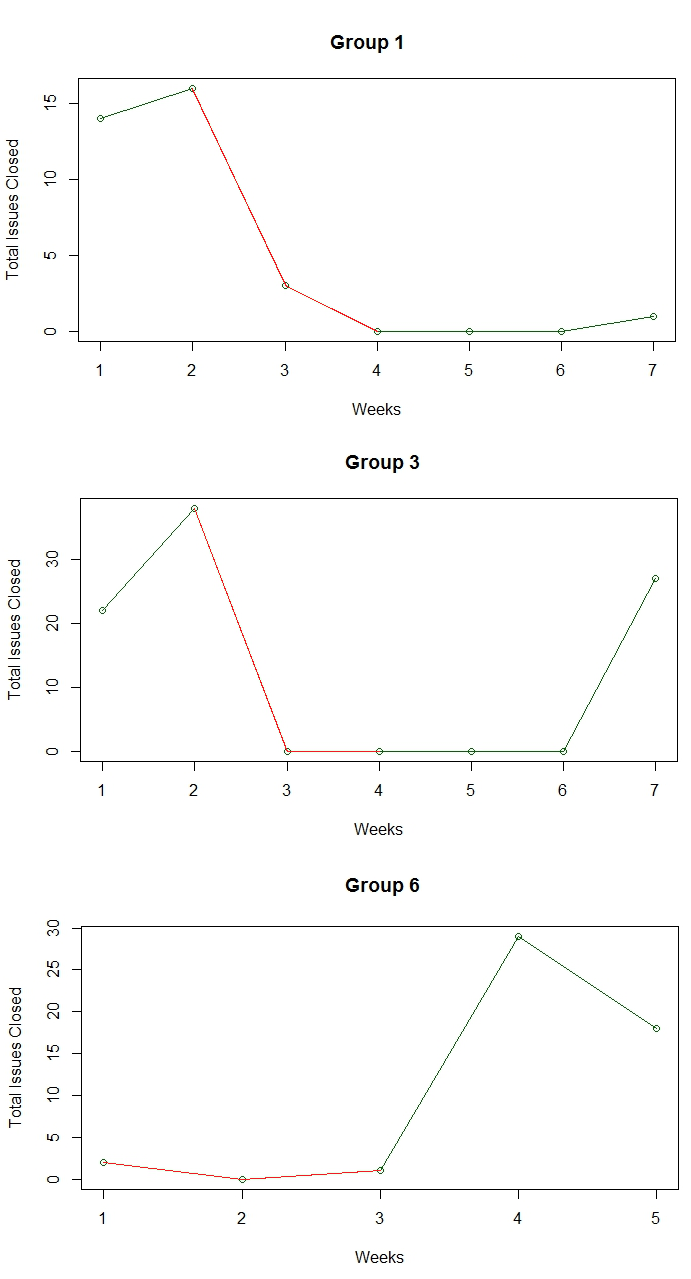
\includegraphics[width=8cm]{img/closedDetect}
\caption{Early Bad Smell Detection on Issues Closed}
\label{fig:closedDetect}
\end{figure}

\section{Conclusion}\label{sec:conclusion}

Having the entire class work collectively on separate group projects through a public platform like GitHub allows for unique and meaningful reflections that can be observed from our public artifacts. These public artifacts are left from nearly every single interaction each group member has with their project's GitHub, and because of this using GitHub provides for an interesting documentable collaboration timeline. 

Through this collaboration timeline we are able to inspect both our peers, and our own progress to develop trends of collaboration. In this report we have identified ten different feature extractions from this public GitHub data, and for each feature we have created meaningful graphs that accurately represent their data. We have also commented on these feature extractions insofar as pointing out what they represent, and if they show good or bad collaboration for a given group.

Furthermore, and perhaps more importantly, using this data we can see where groups failed to work together. To this end, we have identified seven different bad smells which commented on our feature extractions, detailing where groups failed and how they did so. In doing this we have left detailed critiques on observable group progress which led to poor project collaboration.

Finally, we also laid the ground work for an early bad smell detector. While we didn't go as far as creating an algorithm which takes as input a group's public information at a given time to output which bad smells they are developing, we did perform significant analysis. Our analysis focused on the current data sets we had access to and identified where one could identify the bad smells early.

Yet, perhaps the most important and repeatable aspect of this project we noticed when working with our GitHub artifacts dealt with GitHub as a platform for collaboration. Ultimately, we determined that GitHub is an excellent team collaboration platform, which allows for not only a history of source control, but also a slew of critical teamwork features like issues, milestones, comments, and labels. When used properly GitHub is without a doubt a superb collaboration platform; however, the trick lies in learning how to use it properly.

\bibliographystyle{abbrv}
\bibliography{citations}

%\balancecolumns 

\end{document}